\chapter{Introduction} \label{introduction}

Orbital is the School of Computing`s self-driven programming summer experience. It is designed to give first-year students the opportunity to self-learn and build something useful. It is designed as a 4 modular credit (MC) module that is taken pass/fail (CS/CU) over the summer\cite{citation0}. With its focus on hands-on experience, it has been catching more and more attention and an increasing number of first-year students are joining the program to code something useful and interesting. During the academic year of 2015-2016, more than 250 students completed Orbital program with 20 advisers evaluating these teams.

Team is the basic unit in Orbital to start a project, submit project log and evaluate other teams. To express their interests in Orbital program, students will have to register in Skylab first. They can sign up as a team of two students if they have a partner in mind. If at the time of registration they do not have any one in mind whom they can partner with during the summer, they can sign up as individual first and a match making session is going to be conducted before Orbital program officially starts to help them find a good partner.

After registration, for those who are accepted into Orbital program, they will start working on their project ideas and at 3 different timings(checkpoints) throughout the summer, they will need to report their progress by submitting their project's README and project log. And then assigned peer teams(each team will be assigned about 3 peer teams) will be giving feedback regarding the submission and the application built by the team. At the same time, there will be an adviser who will overlook the whole process and provide evaluation of a team's submission as well. After the submissions and evaluations are done, a feedback is expected from a team to its peer teams and its adviser regarding the quality of evaluations received. An illustration of the whole workflow is as Figure~\ref{fig:EvaluationWorkflow}.

\begin{figure}[h]
  \centering
  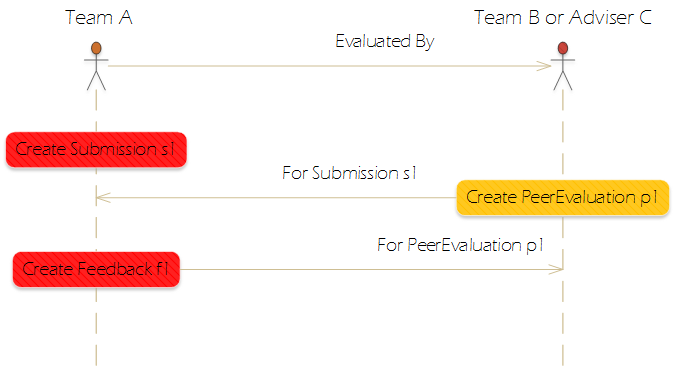
\includegraphics[width=0.85\textwidth]{Images/Skylab_Evaluation_Workflow.png}
  \caption{Illustration of evaluation workflow in Skylab}
  \label{fig:EvaluationWorkflow}
\end{figure}

The nature of Orbital defines the scope of Skylab —-- a development project built for administrators, facilitators, advisers, mentors and students and potential students in Orbital program. It also provides students with a real-life Software Engineering training ground to learn and sharpen programming and system design skills.

\section{Challenges}

\subsection{Tight deadlines}

As the implementation of Skylab was started only at March of 2015 and students started using the system at May of 2015, there is not much time for development. In fact, many features could only be delivered and put into production right before students are using. Chasing deadlines and fixing urgent issues during implementation, especially in the summer when students were actively using Skylab, not only brought a lot of pressure to me but also led to difficulties in system design. Some decisions were made with compromise to deadlines, leaving potential problems for later implementation of Skylab.

\subsection{System design}

Skylab is built using Ruby on Rails, a mature convention-over-configuration web framework. So the first challenge is to get familiar with the conventions and recommended ways of doing things in Rails community. Then Skylab can be designed into a web application on the top of main-stream philosophy in Rails community. Another issue with the design of Skylab is that this is the first time for the developer of Skylab to design such an application from ground up, without any guidance from any experienced Ruby on Rails developers. Therefore, it is all about trial-and-error and explore my own way. Reading books and browsing online tutorials helped a lot and luckily there are plenty of resources about Ruby on Rails development due to its popularity.

\subsection{Evolving requirements}

Although the scope of the project is very clear and well-defined, changes in requirements are expected and did happen a lot due to evolving features of Skylab project and Skylab users' feedback. The challenge is to cope with all changes and sometimes adjustments to the design of system have to be made to accommodate for extensions and new requirements. Therefore agility in development and adaptability of the system is expected.

\subsection{Data migration}

Sometimes schema migration is required as a result of change in requirements. Therefore, dealing with old data and migration of data without affecting the use of application is another challenge during the development of Skylab. Extreme attention when migrating is required as data may not be clean enough and careless migration may even cause the system to be unusable for some users.

\subsection{Security}

Security is definitely a very important perspective in web development. Although Rails is handling security well by taking measures against SQL injection, XSS attacks and CSRF attacks, there are still quite some vulnerabilities if not handled well. During development of Skylab, various techniques and practices are adopted to make Skylab more secure and trust-able. What is more, with different roles in Skylab, a role based access control system is in place to permit users to carry out allowed actions only.

\subsection{Coding quality/maintainability}

Although currently there is only one developer constantly contributing to Skylab repository, a good development cycle which is agile enough is not only important to keep track of history and manage different issues but also convenient for developers who may join later to jump in and get started in a short time. Testing is also a very important factor when it comes to long-term maintenance. A continuous integration would also help in catching regression errors in development early and easily. Besides all mentioned above, refactoring is helpful to the maintainability and growth of Skylab.


\section{Importance of work}

As Orbital`s evaluation of students` performance is largely based on evaluations from peers, it is very important to make the evaluation process among students to be smooth and user-friendly. Before Skylab is implemented, students were supposed to copy an HTML template and modify accordingly for their project`s README and log —-- then post the submission in a forum visible to other teams. For peer evaluation, they need to repeat the whole process —-- only that this time the form is a lot more complicated and harder to copy and paste. Advisers on the other hand, have to manually remove critical sections from peer evaluations by all of his/her teams before make it visible to evaluated teams. And the worst part is that admin of Orbital program needs to do these manual work as well —-- only this time the admin has to do for all the teams(more than 100) in Orbital. Even with clear instructions, many submissions and peer evaluations are still in wrong formats and advisers and admin need to manually fix those. Lack of standardization also leads to trouble when trying to compile a consolidated result from submissions and peer evaluations. A lot of time is wasted in the whole process and careless mistakes in copying, modifying and pasting are just inevitable. 

So Skylab is designed and implemented to make life of students, advisers and admins of Orbital program a lot easier with standardization and automation of many procedures in Orbital program. So students can just save a lot of time and effort now by simply filling required forms and clicking the ``Submit'' button instead of copying an HTML form, modifying, pasting and finally posting as a post in a forum; advisers do not have to manually take out critical sections from peer evaluation and republish posts as the whole process is taken care by the the system; admins can easily overlook and get statistics of evaluation results through admin portal as well.

\section{Objectives}

In this project, I need to:
\begin{itemize}
  \item Enable users to login via NUS OpenID if they have NUS Net IDs already.
  \item Enable users to login via combination of email and password for those who do not have NUS Net IDs and also serve as a backup solution to NUS OpenID login.
  \item Enable ``Forget password'' feature for those who forget their password to reset their passwords.
  \item Enable users to register for Orbital program as a team.
  \item Enable users to register for Orbital program as an individual and recommend potential good partners based on their interested topics.
  \item Enable students to edit their own team's details including ``Team Name'' and ``Project Level''.
  \item Enable students to submit for Milestones or edit their previous submissions. Besides, students in the same team should be able to see changes made by teammates(For example, Team A is supped to be evaluated by Team B, Team C and Team D. Then Team B, Team C and Team D are evaluator teams to Team A and Team A is the evaluated Team to all 3 teams).
  \item Enable assignment of evaluation relationship among teams. Each team will be assigned 3 teams as evaluators.
  \item Enable students to view submissions from teams that they should evaluate(For example, Team A is supposed to evaluate Team B and Team C; Then students in Team A should be able to view submissions from Team B and Team C).
  \item Enable students to evaluate submissions from teams that they are evaluating.
  \item Enable students to view peer evaluations from peer teams and their adviser(For example, Team B is supposed to be evaluated by Team A and Team C; Then students in Team B should be able to view peer evaluations submitted by Team A and Team C for Team B). For public part of a peer evaluation, students can see response with name of the team that submitted that evaluation; As for private part, students can only see a compilation of all private-part responses without team names.
  \item Enable students to submit feedback regarding the evaluations received(For example, Team B is supposed to be evaluated by Team A and Team C; Then students in Team B should be able to submit feedback to Team A and Team C regarding peer evaluations received from each team).
  \item Enable advisers to view a list of all teams under his/her supervision and edit any of these team's details including ``Team name'', ``Project Level'' and ``Has Dropped''.
  \item Enable advisers to submit evaluations to submissions from teams he/she supervises.
  \item Enable advisers to view feedback from his/her teams.
  \item Enable advisers to view a list of all teams and students in the current cohort.
  \item Enable advisers to view, edit and delete evaluation relationships among teams he/she supervises.
  \item Enable administrators to view, edit and delete any users, students, advisers, mentors, administrators, milestones and evaluation relationships.
  \item Enable administrators to login as any user into the system to debug and oversee things.
  \item Enable listing of all staff of Orbital program and display of their public profiles.
  \item Enable listing of all teams that passed Orbital program and display of the team's basic information.
  \item Add notion of cohort to Orbital program so that Skylab can serve for Orbital program for different cohorts.
  \item Enable admins, mentors and admins to batch send reminder emails to students and keep a history of past emails sent for checking.
\end{itemize}

\section{Outline}

In this report, I will discuss various accomplishments I have done in the development of Skylab. Chapter~\ref{background} will be an overview of current architecture of Skylab, and methodologies I employed during the development. Chapter~\ref{workflow} will be talking about solutions to problems in the implementation of registration and evaluation process. Admin portal will be discussed in details in Chapter~\ref{adminportal}. Chapter~\ref{publicprofile} will be focused on implementation of public profiles of staff and projects in Skylab. Then security related issues such as user authentication and access control will be discussed in Chapter~\ref{security}. Chapter~\ref{testing} is about how testing is done during the development of Skylab to ensure correct behaviors of various functionality and also feedback received from the focus group meeting with advisers in Orbital program. Last but not least, a summary of work and an overlook of future development will come in Chapter~\ref{conclusionandfuturework}.
